Recall from section 7.2
\begin{dgroup}[]
	\begin{dmath}[]
		H=H_0+V
	\end{dmath}
	\begin{dmath}[]
		S_{\beta\alpha}=\delta\left( \beta-\alpha \right)
		-\frac{i}{\hbar}\int_{\mathbb{R}}^{}\! \dd{t_1}\, e^{-\frac{i}{\hbar}t_1\left( E_{\alpha}-E_{\beta} \right)}\mel{\psi_{\beta}^{0}}{V}{\psi_{\alpha}^{0}}
		-\frac{i}{\hbar}\int_{-\infty}^{\infty}\dd{t_1}\, e^{-\frac{i}{\hbar}t_1\left( E_{I}+\hbar\omega_i-E_{F}-\hbar\omega_f \right)}\left( \frac{2e^2\hbar\pi}{m\sqrt{\omega_i\omega_f}}\vtr{\upepsilon}\cdot \vtr{\upepsilon}^{*}\mel{F}{\ldots}{F} \right)
	\end{dmath}
\end{dgroup}
golden rule (sec 4.2/4.3)
Transition rate $\frac{2\pi}{\hbar}\abs{T}^2\rho$
cross section $\dv{\sigma}{\Omega}$ (final photon energy $\hbar\omega_f+a\left( \hbar \omega_f \right)$)
\begin{itemize}
	\item divide by flux $v=c$ (section 6.1)
	\item nr. states
		\begin{dgroup}[]
			\begin{dmath}[]
				\frac{\rd^3 \vtr{k}}{\left( 2\pi \right)^3}=\frac{k^2 \dd{k}\dd{\Omega}}{\left( 2\pi \right)^3}=\frac{\omega_{f}^{2}\dd{\Omega}}{\left( 2\pi \right)^3 c^3 \hbar}\rd{\left( \hbar\omega_f \right)}
			\end{dmath}
			\begin{dmath}[]
				\rho\left( \omega_f \right)=\frac{\omega_{f}^{2}\dd{\Omega}}{\left( 2\pi \right)^3 c^3 \hbar}
			\end{dmath}
		\end{dgroup}
\end{itemize}
\begin{dgroup}[]
	\begin{dmath}[]
		\dv{\sigma}{\Omega}=\frac{1}{c}\frac{2\pi}{\hbar}\underbrace{\frac{\omega_{f}^{2}}{\left( 2\pi \right)^3 c^3\hbar}}_{\rho\left( \omega_f \right)}\abs{T}^2
		=\frac{e^4}{m^2c^4}\frac{\omega_f}{\omega_i}\abs{\vtr{\upepsilon}_i\cdot \vtr{\upepsilon}_{f}^{*}\mel{F}{e^{i\vtr{r}\cdot \left( \vtr{k}_i-\vtr{k}_f \right)}}{I}}^2
	\end{dmath}
	\begin{dmath}[]
		\left( \frac{\alpha\hbar}{mc} \right)^2=r_{0}^{2}
	\end{dmath}
	\begin{dsuspend}
		(classical electron radius)
	\end{dsuspend}
\end{dgroup}
However, there are further contributions of order $\alpha^2\sim e^4$
golden rule (sec 4.2/4.3)
Transition rate $\frac{2\pi}{\hbar}\abs{T}^2\rho$

cross section $\dv{\sigma}{\Omega}$ (final photon)\ldots


\subsection{2nd order contribution}
for $T_{\beta\alpha}$
\begin{figure}[]
	\begin{center}
		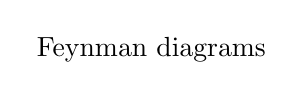
\begin{tikzpicture}[]
			\node[] (a) at (0,0) {Feynman diagrams};
		\end{tikzpicture}
	\end{center}
	\caption{}
	\label{fig:}
\end{figure}
\begin{dgroup}[]
	\begin{dmath}[]
		S_{\beta\alpha}=\ldots
		\left( -\frac{i}{\hbar} \right)^2
		\int_{-\infty}^{\infty}\!\dd{t_1}\int_{-\infty}^{t_1}\! \dd{t_2}\sum_{\gamma}^{}e^{-\frac{i}{\hbar}t_1 \left( E_{\gamma}-E_{\beta} \right)}e^{-\frac{i}{\hbar}t_2\left( E_{\alpha}-E_{\gamma} \right)}V_{\beta\gamma}V_{\gamma\alpha}
	\end{dmath}
\end{dgroup}
In our case
\begin{dgroup}[]
	\begin{dmath}[]
		\left( -\frac{i}{\hbar} \right)^2\int_{-\infty}^{\infty}\! \dd{t_1}\int_{-\infty}^{t_1}\dd{t_2}\int_{}^{}\mkern-26mu\sum_{}^{}\dd{N}\, e^{-\frac{i}{\hbar}\left( E_N -E_F\right)t_i}e^{-\frac{i}{\hbar}\left(E_I-E_N  \right)t_2}\left( \frac{e}{mc} \right)^2\cdot 
		\int_{}^{}\frac{\rd^3 \vtr{k}}{\left( 2\pi \right)^3}\int_{}^{}\frac{\rd^3 \vtr{k}'}{\left( 2\pi \right)^3}\sum_{\lambda\lambda'}^{}\mel{F,P\left( \omega_f,\lambda_f \right)}{\hat{a}_k\vtr{p}\cdot \vtr{\upepsilon}_k e^{i\vtr{k}\cdot \vtr{r}-i\omega t_1+\hat{a}_{k}^{\dagger}\vtr{p}\cdot \vtr{\upepsilon}_{k}^{*}e^{-i\vtr{k}\cdot \vtr{r}+i\omega t_1}}}{N}
		\cdot \mel{N}{\hat{a}_{k'}\vtr{p}\cdot \vtr{\upepsilon}_{k'}e^{i\vtr{k}'\cdot \vtr{r}-i\omega' t_2}+\hat{a}_{k'}^{\dagger}\vtr{p}\cdot \vtr{\upepsilon}_{k'}^{*} e^{-i\vtr{k}' j \vtr{r}+i\omega' t_2}}{I, 1\left( k_i,\lambda_i \right)}
	\end{dmath}
	\begin{dsuspend}
		need $1$ $\hat{a}\left( k_i,\lambda_i \right)$ and one $\hat{a}^{\dagger}\left( k_f,\lambda_f \right)$
	\end{dsuspend}
	\begin{dmath}[]
		=\ldots
		= \mel{F}{\hat{a}_{k_f}^{\dagger}\ldots }{N}\mel{N}{\ldots \hat{a}_{k_i}}{I}
		+\mel{F}{\hat{a}_{k_i}\ldots}{N}\mel{N}{\ldots \hat{a}_{\dagger}^{k_f}}{I}
	\end{dmath}
\end{dgroup}
Kramers Heisenberg formula

\begin{dmath}[]
	\dv{\sigma}{\Omega}=\left( \frac{\alpha\hbar}{mc} \right)^2\frac{\omega_f}{\omega_i}\abs{\vtr{\upepsilon}_i\vtr{\upepsilon}_f^{*}\delta_{FI}
	+\sum_{N}^{}\mel{F}{\vtr{p}\cdot\upepsilon_{f}^{*}}{N}\mel{N}{\vtr{p}\cdot \vtr{\upepsilon}_i}{I}
	+\frac{\mel{F}{\vtr{p}\cdot \vtr{\upepsilon}_i}{N}\mel{N}{\vtr{p}\cdot \vtr{\upepsilon}_{f}^{*}}{I}}{m\left( E_{I}-\hbar\omega_f-E_N \right)}
}
\end{dmath}
$\to$ limiting cases
\paragraph{Rayleight scattering}
elastic scattering 
\begin{dgroup}[]
	\begin{dmath}[]
		\ket{I}=\ket{F}
	\end{dmath},
	\begin{dmath}[]
		\omega_i=\omega_f
	\end{dmath}
	\begin{dmath}[]
		\hbar\omega\ll E_{I}-E_{N}
	\end{dmath}
\end{dgroup}
combine $\vtr{\upepsilon}_i\cdot \vtr{\upepsilon}_f$ with other terms
\begin{dgroup}[]
	\begin{dmath}[]
		\mel{I}{\vtr{\upepsilon}_i\upepsilon_{f}^{*}}{I}
		=\frac{1}{i\hbar}\mel{I}{\comm{\vtr{x}\cdot \vtr{\upepsilon}_i}{\vtr{p}\cdot \vtr{\upepsilon}_{f}^{*}}}{I}
		=\frac{1}{i\hbar}\sum_{N}^{}\left( \mel{I}{\vtr{x}\cdot \vtr{\upepsilon}_i}{N}\mel{N}{\vtr{p}\cdot \vtr{\upepsilon}_{f}^{*}}{I}-\mel{I}{\vtr{p}\cdot \vtr{\upepsilon}_{f}^{*}}{N}\mel{N}{\vtr{p}\cdot \vtr{\upepsilon}_f^{*}}{I} \right)
	\end{dmath}
\end{dgroup}
$\to$ put everything together:
\begin{dgroup}[]
	\begin{dmath}[]
		\frac{1}{E_{N}-E_{I}}+\frac{1}{E_{I}-E_{N}+\pm \hbar\omega}
		=\mp \frac{\hbar\omega}{\left( E_{I}-E_{N} \right)^2}+\frac{\left( \hbar\omega \right)^2}{\left( E_{I}-E_{N} \right)^2}+\ldots
	\end{dmath}
	\begin{dmath*}[]
		\dv{\sigma}{\Omega}=r_{0}^{2}\frac{\left( \hbar\omega \right)^4}{m^2}
		\abs{\sum_{N}^{}\frac{\mel{I}{\vtr{p}\cdot \vtr{\upepsilon}_{f}^{*}}{N}\mel{N}{\vtr{p}\cdot \vtr{\upepsilon}_i}{I}}{\left( E_{I}-E_{N} \right)^2}+ \hiderel{\leftrightarrow}
	}^2
	\end{dmath*}
	\begin{dsuspend}
		$r_{0}^{2}$ classical $e$-radius, $\omega^4$ blue sky red sunset
	\end{dsuspend}
\end{dgroup}
\paragraph{Thomson scattering}
\begin{dgroup}[]
	\begin{dmath}[]
		\hbar \omega_i\gg E_{N}-E_{I}
	\end{dmath}
	\begin{dsuspend}
		(large compared to bindig energy $\leadsto$ scattering off ``free'' electrons)
	\end{dsuspend}
	\begin{dmath}[]
		\dv{\sigma}{\Omega}=r_{}^{2}\abs{\vtr{\upepsilon}_i\cdot \vtr{\upepsilon}_f}^2
	\end{dmath}
	\begin{dsuspend}
		for unpolarized photons
	\end{dsuspend}
	\begin{dmath}[]
		\frac{1}{2}\sum_{\lambda_i\lambda_f}^{}\varepsilon_{i}^{a}\left( k_i,\lambda_i \right)\left( \varepsilon_{f}^{} \right)^a\left( k_f,\lambda_f \right) \varepsilon_{i}^{b}\left( \varepsilon_{f}^{*} \right)^b
		=\frac{1}{2}\left( \delta_{ab}-\frac{k_{i}^{a}k_{i}^{b}}{k_{i}^{)}} \right)\left( \delta_{ab}-\frac{k_{f}^{a}k_{f}^{b}}{k_{f}^{2}} \right)
		=\frac{1}{2}\left( 1+\cos^2\theta \right)
	\end{dmath}
	\begin{dsuspend}
		with 
	\end{dsuspend}
	\begin{dmath}[]
		\theta=\sphericalangle \left( \vtr{k}_i,\vtr{k}_f \right)
	\end{dmath}
	\begin{dmath}[]
		\sigma=\int_{}^{}\dd{\cos\theta}\, 2\pi r_{0}^{2}\left( 1+\cos^2\theta \right)
		=\frac{8\pi}{3}r_{0}^{2}
	\end{dmath}
\end{dgroup}
\paragraph{Resonances}
What if $E_{N}\sim E_{I}+\hbar\omega_i$

so far : neglected finite lifetime of $E_N$, $\tau_N=\frac{\hbar}{\Gamma_N}$

time evolution 

\begin{dgroup}[]
	\begin{dmath}[]
		e^{-\frac{i}{\hbar}E_{N}t}e^{-\tau_N t}
		=e^{-\frac{i}{\hbar}t\left( E_{N}-i\Gamma_N \right)}
	\end{dmath}
	\begin{dsuspend}
		with $\Gamma_N$ that one cannot neglect
	\end{dsuspend}
	\begin{dmath}[]
		\abs{T}^2\approx\abs{\frac{1}{E_{I}-E_{N}+i\Gamma_N}}^2
		=\frac{1}{\left( E_{I}-E_{N} \right)^2+\Gamma_{N}^{2}}
	\end{dmath}
\end{dgroup}
\chapter{Relativistic QM}
Will wry to find relativistic generalization of Schrödinger as single-particle equation ($\to$ we will fail) but will be basis of relativistic ($2nd$ quantized field theory)
Rel: Cannot fix number of particles
\section{Klein-Gordon equation (KGE)}
Consider dfree scalar particle 
\begin{dgroup}[]
	\begin{dmath}[]
		X^{\mu}\to X^{\mu'}=\Lambda_{\; \nu}^{\mu}x^{\nu}
	\end{dmath}
	\begin{dmath}[]
		\phi(x)\to \phi'\left( x' \right)=\phi(x)=\phi\left( \Lambda^{-1} x' \right)
	\end{dmath}
\end{dgroup}
Now start from
\begin{dgroup}[]
	\begin{dmath}[]
		E^{2}=m^2c^4+\vtr{p}^2c^2
	\end{dmath}
	\begin{dsuspend}
		(\emph{not} $E=\frac{p^2}{2m}$)
	\end{dsuspend}
	\begin{dmath}[]
		E\to i\hbar \pdv{}{t}
	\end{dmath}
	\begin{dmath}[]
		\vtr{p}=-i\hbar\vtr{\nabla}
	\end{dmath}
	\begin{dmath}[]
		\left( -\hbar^2\pddv{}{t} \right)\phi(\vtr{x},t)
		=\left( m^2c^4-\hbar c^2\vtr{\nabla}^2 \right)\phi(x,t)
	\end{dmath}
	\begin{dsuspend}
		in covariant form:
	\end{dsuspend}
	\begin{dmath}[]
		\partial_{\mu}\partial^{\mu}+\frac{m^2c^2}{\hbar^2}\phi(x)=0
	\end{dmath}
	\begin{dmath}[]
		\partial_{\mu}=\pdv{}{x^{\mu}}=\left( \frac{1}{c}\pdv{}{t},\vtr{\nabla} \right)
	\end{dmath}
	\begin{dmath}[]
		\partial^{\mu}=\left( \frac{1}{c}\pdv{}{t}-\vtr{\nabla} \right)
	\end{dmath}
\end{dgroup}
